\documentclass[11pt,a4paper]{article}
\usepackage[utf8]{inputenc}
\usepackage{amsmath,amsfonts,amssymb}
\usepackage{graphicx}
\usepackage{geometry}
\geometry{margin=1in}
\usepackage{booktabs}
\usepackage{hyperref}
\usepackage{float}
\usepackage{xcolor}

\definecolor{darkbg}{HTML}{0d121f}
\definecolor{lighttext}{HTML}{e2e8f0}
\definecolor{primary}{HTML}{8b5cf6}
\definecolor{secondary}{HTML}{0dd5c5}

\pagecolor{darkbg}
\color{lighttext}

\hypersetup{
    colorlinks=true,
    linkcolor=secondary,
    urlcolor=secondary
}

\title{\textbf{EE3621: Digital Signal Processing} \\ \Large Lecture 11: FIR Filter Design --- Frequency Sampling \& Optimal Methods \\ \large (III B.Tech EEE)}
\author{Lecture Notes (40-Minute Plan)}
\date{}

\begin{document}

\maketitle

\section{Lecture Plan (40 Minutes Breakdown)}
\begin{itemize}
    \item \textbf{00:00 -- 05:00 (5 mins):} Introduction to Frequency Sampling Design.
    \item \textbf{05:00 -- 12:00 (7 mins):} Transition Sample Optimization.
    \item \textbf{12:00 -- 20:00 (8 mins):} Parks-McClellan (Remez Exchange) Algorithm and Alternation Theorem.
    \item \textbf{20:00 -- 25:00 (5 mins):} Design Formulas (Kaiser, Herrmann-Rabiner).
    \item \textbf{25:00 -- 30:00 (5 mins):} FIR Filter Types (I, II, III, IV) and their constraints.
    \item \textbf{30:00 -- 35:00 (5 mins):} Worked Example: 15-tap Equiripple Bandpass Filter.
    \item \textbf{35:00 -- 40:00 (5 mins):} FIR vs IIR Comparison and Checkpoint Questions.
\end{itemize}

\noindent\rule{\textwidth}{0.5pt}

\section{Frequency Sampling Method}

\begin{figure}[H]
    \centering
    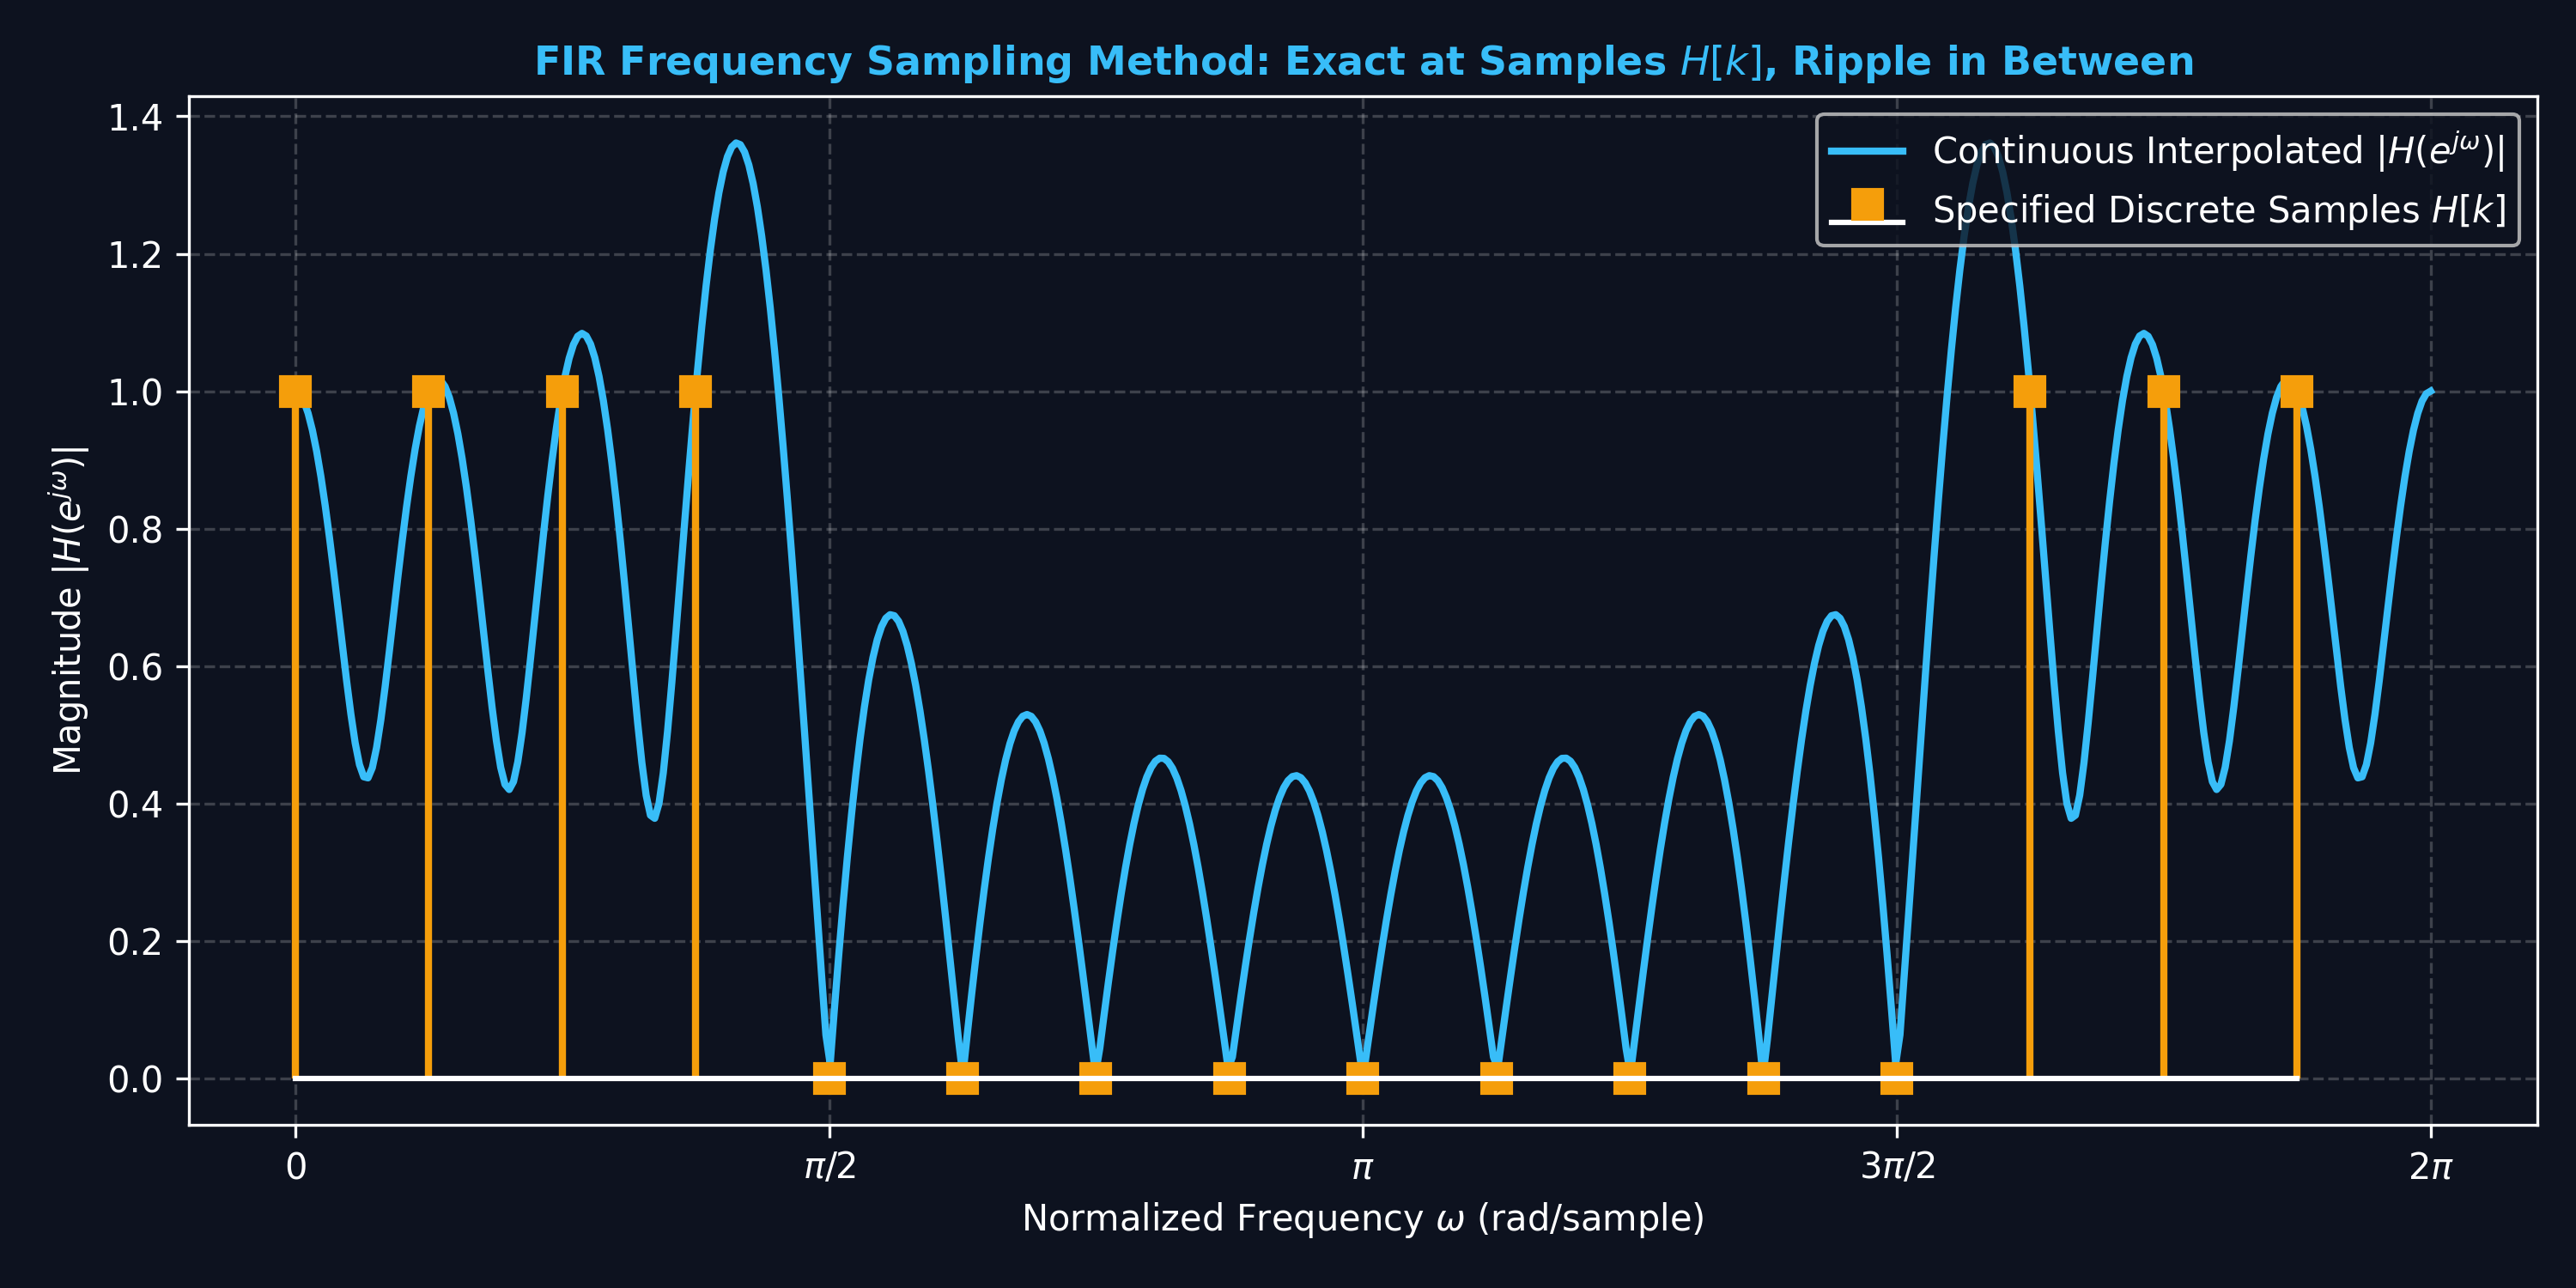
\includegraphics[width=0.85\textwidth]{images/freq_sampling_discrete_grid.png}
    \caption{FIR Frequency Sampling Method: Exact Interpolation on Discrete Target Grid Points $H[k]$.}
\end{figure}

\begin{figure}[H]
    \centering
    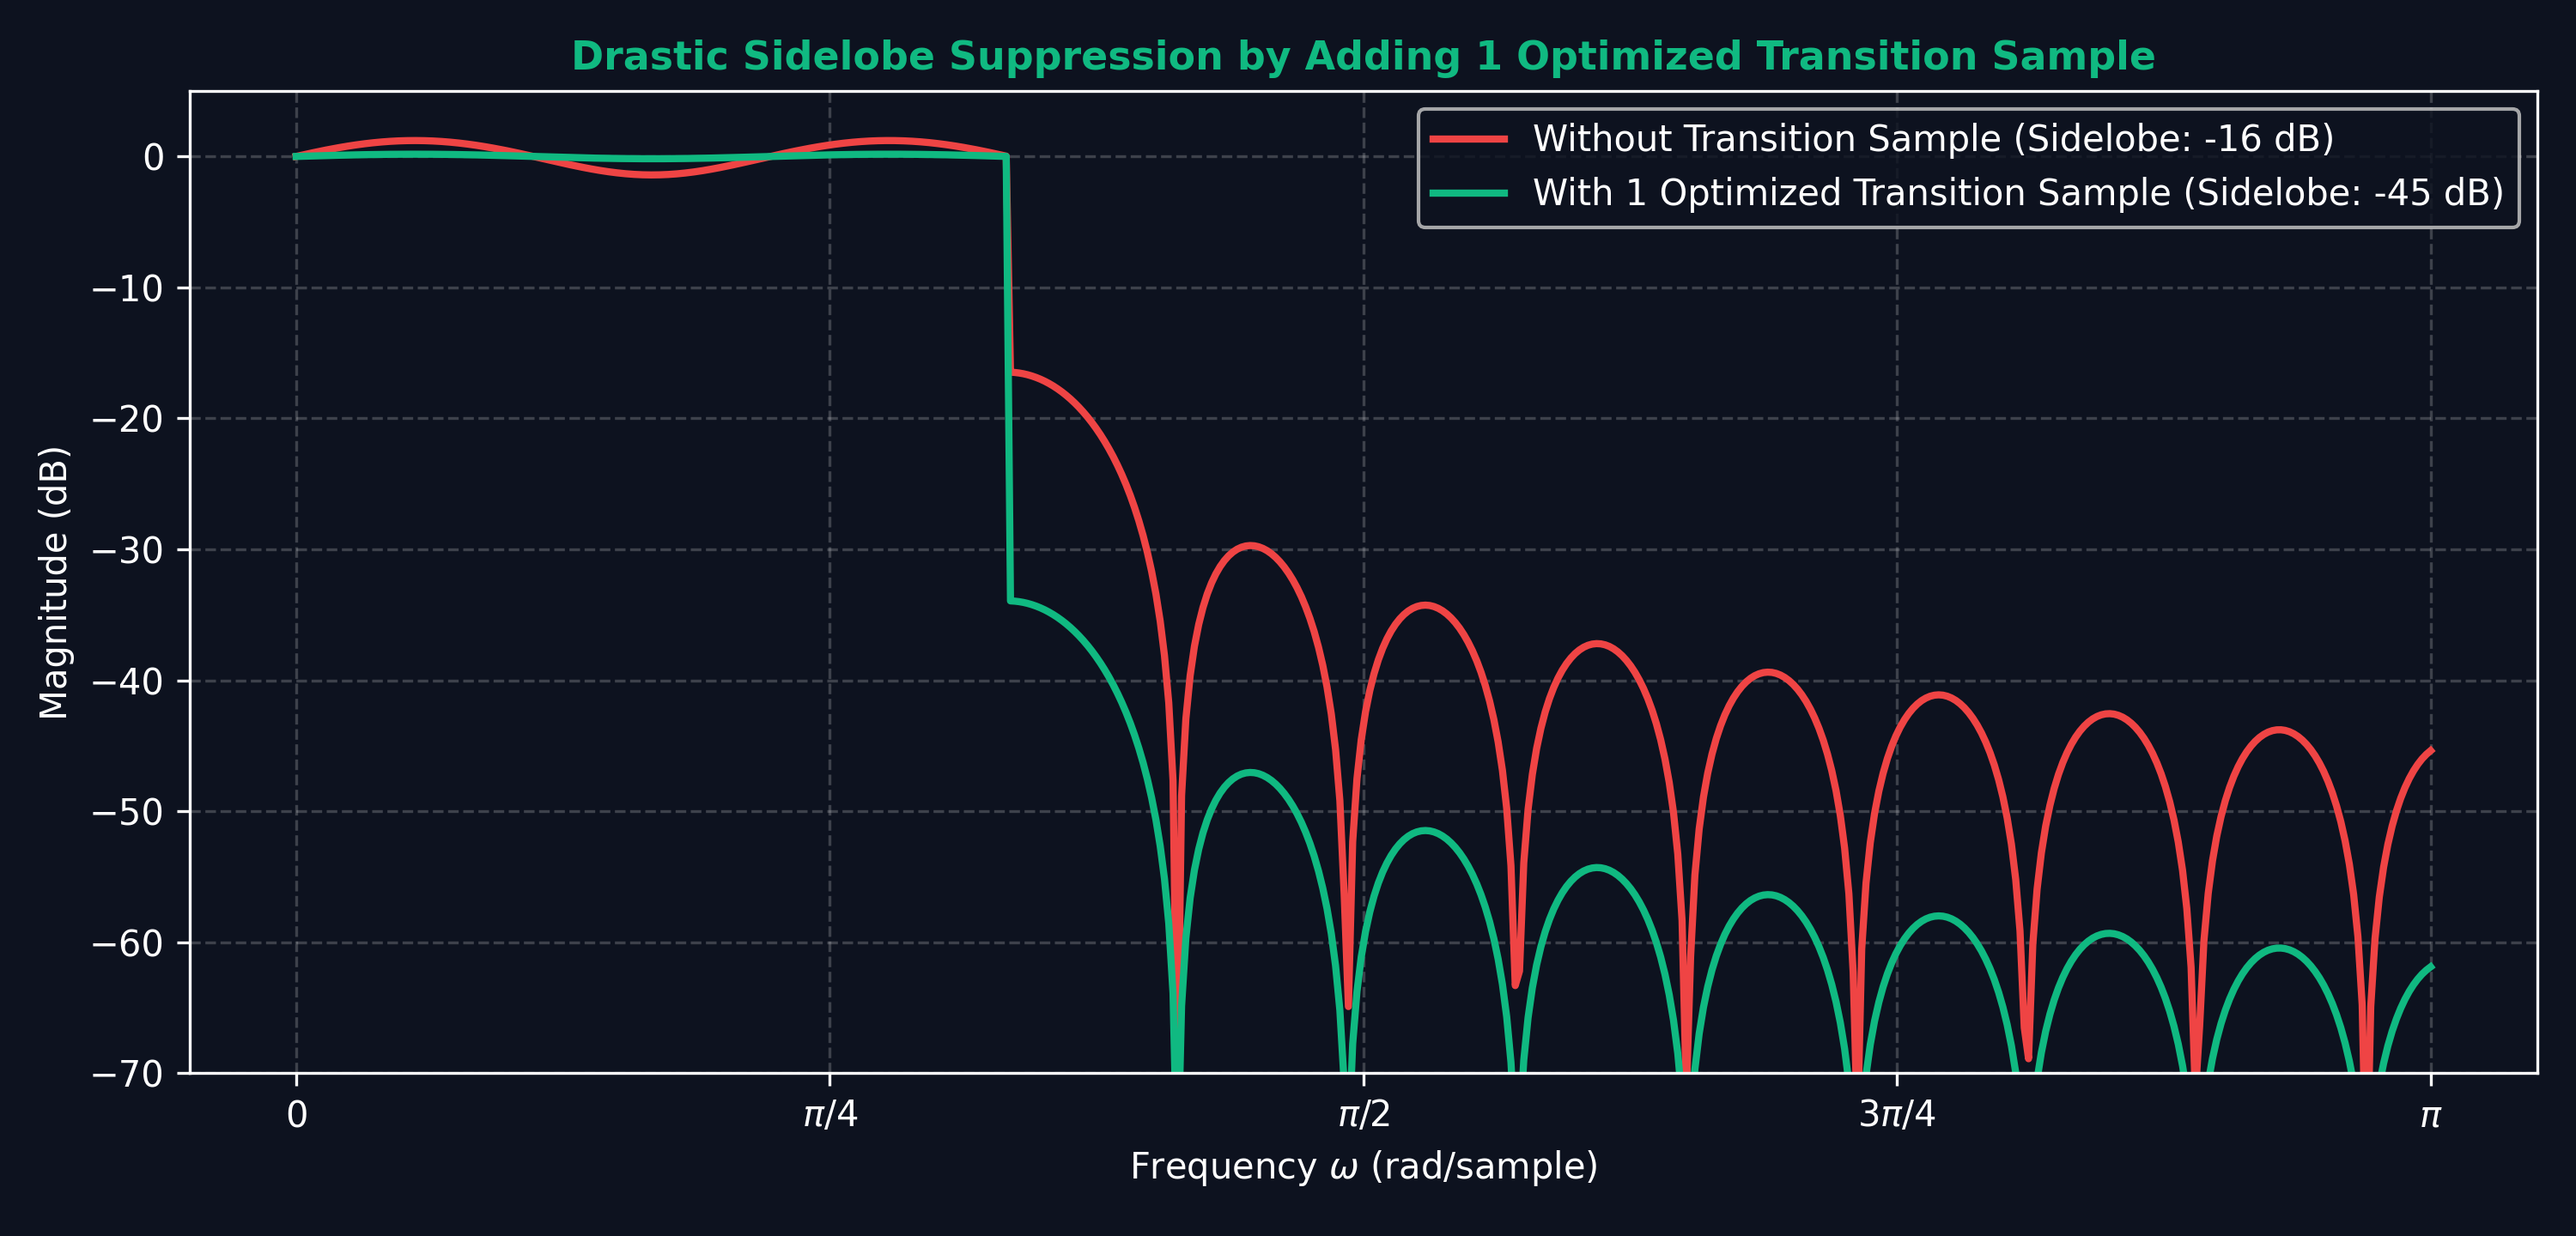
\includegraphics[width=0.85\textwidth]{images/transition_band_optimization.png}
    \caption{Sidelobe Optimization: Suppressing Stopband Ripples to $-45\text{ dB}$ via Optimized Transition Samples.}
\end{figure}

\begin{figure}[H]
    \centering
    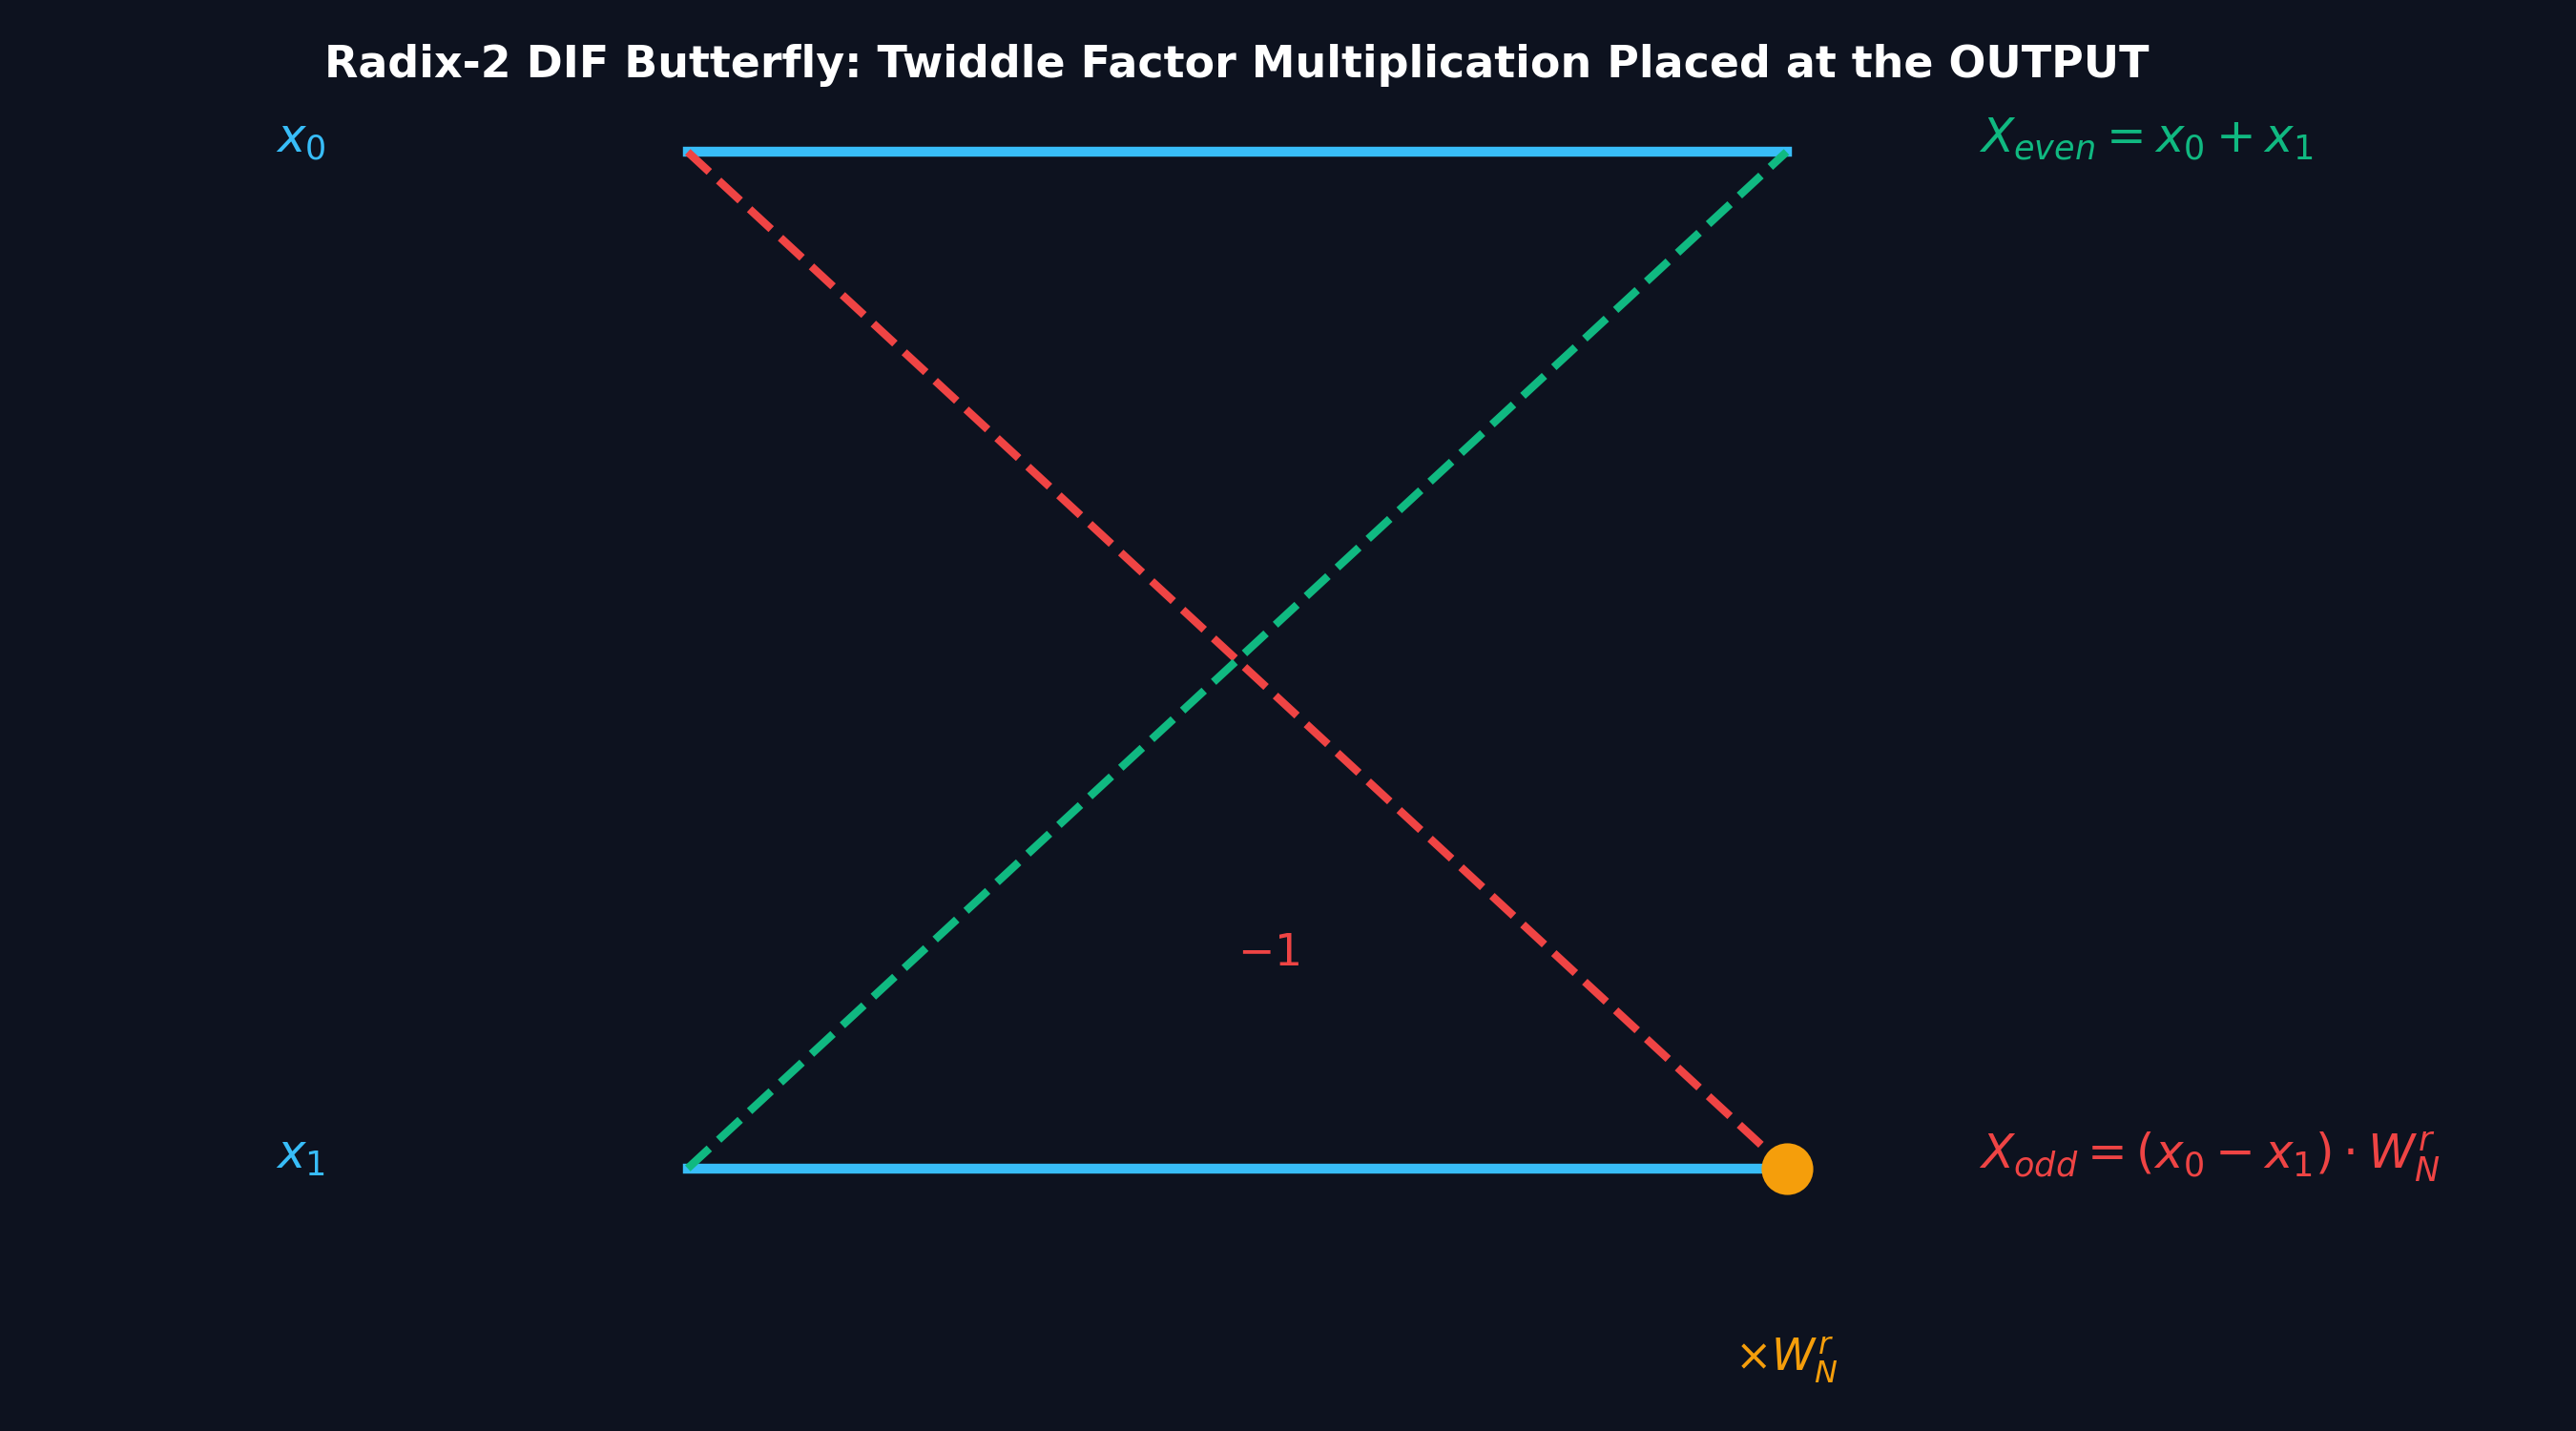
\includegraphics[width=0.75\textwidth]{images/dif_butterfly.png}
    \caption{Radix-2 Decimation-in-Frequency (DIF) Butterfly Structure with Output Twiddle Multiplication.}
\end{figure}

The frequency sampling method is a direct way to design FIR filters. Instead of manipulating the impulse response in the time domain, we specify the desired frequency response exactly at $N$ equally spaced points in the frequency domain.

\subsection{Concept and Formulation}
Let the desired continuous frequency response be $H_d(\omega)$. We sample this response at $N$ equally spaced frequencies in the range $0 \le \omega < 2\pi$:
\begin{equation}
\omega_k = \frac{2\pi k}{N}, \quad k = 0, 1, \dots, N-1
\end{equation}

The sampled frequency response is defined as:
\begin{equation}
H[k] = H_d\left(\frac{2\pi k}{N}\right)
\end{equation}

The impulse response $h[n]$ of the FIR filter is obtained by taking the $N$-point Inverse Discrete Fourier Transform (IDFT) of $H[k]$.

\subsection{Derivation of Impulse Response}
We start with the IDFT definition:
\begin{equation}
h[n] = \frac{1}{N} \sum_{k=0}^{N-1} H[k] e^{j \frac{2\pi}{N} kn}
\end{equation}
\begin{equation}
h[n] = \frac{1}{N} \sum_{k=0}^{N-1} H[k] W_N^{-kn}
\end{equation}
where $W_N = e^{-j 2\pi / N}$ is the twiddle factor.

Let's expand the summation carefully to show the symmetry properties. Assuming $H[k]$ is conjugate symmetric (since $h[n]$ must be real):
\begin{equation}
H[N-k] = H^*[k]
\end{equation}

We can split the summation into the DC component, the Nyquist component (if $N$ is even), and the conjugate symmetric pairs. For $N$ odd:
\begin{equation}
h[n] = \frac{1}{N} H[0] + \frac{1}{N} \sum_{k=1}^{(N-1)/2} \left[ H[k] e^{j \frac{2\pi}{N} kn} + H[N-k] e^{j \frac{2\pi}{N} (N-k)n} \right]
\end{equation}
\begin{equation}
h[n] = \frac{1}{N} H[0] + \frac{1}{N} \sum_{k=1}^{(N-1)/2} \left[ H[k] e^{j \frac{2\pi}{N} kn} + H^*[k] e^{-j \frac{2\pi}{N} kn} \right]
\end{equation}

Let $H[k] = |H[k]| e^{j \angle H[k]}$. Then:
\begin{equation}
h[n] = \frac{1}{N} H[0] + \frac{2}{N} \sum_{k=1}^{(N-1)/2} |H[k]| \cos\left(\frac{2\pi}{N} kn + \angle H[k]\right)
\end{equation}

For a linear phase FIR filter, we must impose constraints on $\angle H[k]$. Specifically, for a Type I filter (symmetric, odd $N$), the phase must be:
\begin{equation}
\angle H[k] = - \alpha \frac{2\pi k}{N}
\end{equation}
where $\alpha = \frac{N-1}{2}$.

Substituting this back into the equation:
\begin{equation}
h[n] = \frac{1}{N} H[0] + \frac{2}{N} \sum_{k=1}^{(N-1)/2} |H[k]| \cos\left(\frac{2\pi k}{N} (n - \alpha)\right)
\end{equation}

\textbf{KEY RESULT:} The filter exactly interpolates the specified points at $\omega_k$. However, between the sample points, the frequency response may exhibit significant ripple, especially near the transition band.

\section{Transition Sample Optimization}

The basic frequency sampling method can lead to large ripples between the sample points in the passband and stopband (similar to the Gibbs phenomenon). To mitigate this, we can introduce one or more ``transition samples'' in the transition band.

\subsection{Intuition}
Instead of forcing the frequency response to jump abruptly from 1 to 0 between two adjacent frequency samples, we introduce an intermediate value (e.g., $T_1 = 0.39$).

\subsection{Effect of Transition Samples}
By allowing the transition band to have a non-zero sample, we increase the transition width, but we gain an additional degree of freedom. This degree of freedom can be optimized to minimize the maximum sidelobe level in the stopband.

Example:
For a lowpass filter with $N = 33$, suppose we specify:
\begin{itemize}
    \item Passband: $H[0] = H[1] = H[2] = H[3] = 1$
    \item Transition: $H[4] = T_1$
    \item Stopband: $H[5] = \dots = H[16] = 0$
\end{itemize}

Without $T_1$ (i.e., $T_1 = 0$), the stopband attenuation might only be -20 dB.
By optimizing $T_1$, we can push the stopband attenuation to -40 dB or better. A common optimal value found via linear programming is $T_1 \approx 0.39$.

\section{Parks-McClellan (Remez Exchange) Algorithm}

While frequency sampling is simple, it is not optimal. The window method is also sub-optimal because it minimizes the mean squared error rather than the maximum absolute error. The \textbf{Parks-McClellan algorithm} designs optimal equiripple FIR filters by minimizing the Chebyshev (minimax) error.

\subsection{Chebyshev Approximation Problem Formulation}
Let $H(\omega)$ be the zero-phase frequency response of an FIR filter.
Let $H_d(\omega)$ be the desired frequency response.
Let $W(\omega)$ be a positive weighting function that allows us to specify different error tolerances for different frequency bands.

The weighted error function is defined as:
\begin{equation}
E(\omega) = W(\omega) [H_d(\omega) - H(\omega)]
\end{equation}

The goal is to find the filter coefficients that minimize the maximum absolute error over the closed subset of frequencies $A \subset [0, \pi]$. Mathematically, we want to minimize:
\begin{equation}
\max_{\omega \in A} |E(\omega)|
\end{equation}
This is the minimax or Chebyshev approximation problem:
\begin{equation}
\min_{h[n]} \max_{\omega \in A} W(\omega) |H_d(\omega) - H(\omega)|
\end{equation}

\subsection{Alternation Theorem}
The solution to the Chebyshev approximation problem is characterized by the \textbf{Alternation Theorem}.

\textbf{Theorem:} If $H(\omega)$ is a linear combination of $L$ independent cosine functions (i.e., $H(\omega)$ has $L$ free parameters), then $H(\omega)$ is the unique optimal min-max approximation if and only if the error function $E(\omega)$ exhibits at least $L+1$ extremal frequencies (alternations) in $A$.

At these extremal frequencies $\omega_i$, the error reaches the maximum magnitude but alternates in sign:
\begin{equation}
E(\omega_i) = -E(\omega_{i+1}) = \pm \max_{\omega \in A} |E(\omega)|
\end{equation}

For a Type I FIR filter of length $N$, the number of free parameters is $L = \frac{N+1}{2}$. Thus, the optimal filter must have at least $L+1$ alternations.

\subsection{Remez Algorithm Outline}
The Parks-McClellan algorithm uses the Remez exchange algorithm, an iterative procedure:
\begin{enumerate}
    \item \textbf{(a) Guess extremal frequencies:} Initialize a set of $L+1$ guess frequencies $\omega_i$.
    \item \textbf{(b) Solve for polynomial:} Calculate the optimal maximum error $\delta$ and the polynomial $H(\omega)$ that satisfies $E(\omega_i) = (-1)^i \delta$.
    \item \textbf{(c) Find actual maximum error location:} Evaluate $E(\omega)$ on a dense grid over $A$ to find the actual local maxima of $|E(\omega)|$.
    \item \textbf{(d) Update extremal set:} If the maximum error on the dense grid is greater than $\delta$, update the set of extremal frequencies.
    \item \textbf{(e) Iterate:} Repeat steps (b) through (d) until the extremal frequencies converge.
\end{enumerate}

\subsection{Comparison with Window Method}
\begin{itemize}
    \item \textbf{Optimality:} The equiripple filter has the minimum possible order for a given set of specifications.
    \item \textbf{Error Distribution:} The window method produces larger ripples near the band edges, whereas the equiripple method spreads the error evenly.
    \item \textbf{Complexity:} The window method is analytically simple, while Parks-McClellan requires an iterative numerical solver.
\end{itemize}

\section{Design Formulas}

\subsection{Kaiser Formula}
Kaiser proposed a simple formula to estimate $N$:
\begin{equation}
N \approx \frac{-20 \log_{10}(\sqrt{\delta_p \delta_s}) - 13}{14.6 \Delta f} + 1
\end{equation}
where $\Delta f = \frac{\omega_s - \omega_p}{2\pi}$.

\subsection{Herrmann-Rabiner Formula}
A more accurate formula:
\begin{equation}
N \approx \frac{D_{\infty}(\delta_p, \delta_s) - F(\delta_p, \delta_s) (\Delta f)^2}{\Delta f} + 1
\end{equation}

\section{Type I, II, III, IV FIR Filters}

\subsection{Type I: Symmetric, Odd Length}
$h[n] = h[N-1-n]$. Center of symmetry is an integer. \textbf{Constraints:} No constraints at $\omega = 0$ or $\omega = \pi$. Can be used for any filter type.

\subsection{Type II: Symmetric, Even Length}
$h[n] = h[N-1-n]$. Center of symmetry is a half-integer. \textbf{Constraints:} $H(e^{j\pi}) = 0$. Cannot be used for Highpass or Bandstop filters.

\subsection{Type III: Anti-Symmetric, Odd Length}
$h[n] = -h[N-1-n]$. \textbf{Constraints:} $h[(N-1)/2] = 0$. $H(e^{j0}) = 0$ and $H(e^{j\pi}) = 0$. Cannot be Lowpass or Highpass.

\subsection{Type IV: Anti-Symmetric, Even Length}
$h[n] = -h[N-1-n]$. \textbf{Constraints:} $H(e^{j0}) = 0$. Cannot be Lowpass.

\section{FIR vs IIR Comparison Table}

\begin{table}[H]
\centering
\caption{FIR vs IIR Filters Comparison}
\begin{tabular}{l p{6cm} p{6cm}}
\toprule
\textbf{Feature} & \textbf{FIR Filters} & \textbf{IIR Filters} \\
\midrule
Stability & Always stable & Conditionally stable \\
Phase Linearity & Can have exact linear phase & Cannot have exact linear phase \\
Filter Order (N) & High (20 to 200+) & Low (2 to 10) \\
Design Complexity & High (Iterative PM algorithm) & Low (Bilinear transform) \\
Computational Load & High & Low \\
Feedback & No (Non-recursive) & Yes (Recursive) \\
Implementation & Efficient via FFT & Standard difference equations \\
\bottomrule
\end{tabular}
\end{table}

\section{Worked Example: 15-Tap Equiripple Bandpass Filter}

\textbf{Problem:} Design a 15-tap ($N=15$) optimal equiripple bandpass filter. 
Desired passband: $\omega \in [0.4\pi, 0.6\pi]$.
Stopbands: $\omega \in [0, 0.2\pi]$ and $\omega \in [0.8\pi, \pi]$.
Equal weighting: $W(\omega) = 1$ in all bands.

\textbf{Step-by-step setup:}
\begin{enumerate}
    \item \textbf{Filter Type:} Since $N=15$ (odd) and we want a bandpass filter, we must use a Type I FIR filter.
    \item \textbf{Number of Free Parameters:}
    \begin{equation}
    L = \frac{N+1}{2} = \frac{15+1}{2} = 8
    \end{equation}
    \item \textbf{Alternation Theorem Requirement:}
    The optimal error curve must have at least $L+1 = 9$ alternating extrema.
    \item \textbf{Parks-McClellan Execution:}
    The algorithm picks 9 initial guess frequencies. It solves for the optimal error $\delta$ and the coefficients. Then it evaluates the actual frequency response on a dense grid to find the peaks of the error curve, updating the guess frequencies until convergence.
\end{enumerate}

\textbf{Output:} The PM algorithm returns the 8 independent coefficients $h[0], \dots, h[7]$. The remaining coefficients are found via symmetry: $h[8] = h[6], \dots, h[14] = h[0]$.

\section{Checkpoint Questions}

\begin{enumerate}
    \item \textbf{Q1: Why can't a Type II FIR filter be used to design a highpass filter?} \\
    \textit{Detailed Answer:} A Type II FIR filter has an even number of taps ($N$ is even) and symmetric coefficients. The frequency response evaluation mathematically forces a zero at $\omega = \pi$. A highpass filter must pass the frequency $\omega = \pi$ (i.e., $H(e^{j\pi}) \neq 0$). Since a Type II filter strictly forces the response to be zero at $\pi$, it is physically impossible to use it as a highpass filter.

    \item \textbf{Q2: In the frequency sampling method, why isn't the resulting filter perfect between samples?} \\
    \textit{Detailed Answer:} The frequency sampling method forces the filter's frequency response to perfectly match the desired response only at the specific sample points. Between these sample points, the frequency response is determined by an interpolation formula. Because the desired response often has abrupt discontinuities, interpolating it leads to severe overshoot and ringing between the samples (Gibbs phenomenon).

    \item \textbf{Q3: According to the Alternation Theorem, a length-21 Type I equiripple lowpass filter must have how many alternations?} \\
    \textit{Detailed Answer:} For a Type I filter, the length $N=21$. The number of independent coefficients is $L = (N+1)/2 = 11$. The Alternation Theorem states that the optimal Chebyshev filter must have at least $L+1$ extremal frequencies. Therefore, there must be at least 12 alternations. Physically, this means the error function hits its maximum allowable magnitude and bounces back at least 12 times.
\end{enumerate}

\section{Summary of Key Formulas}

\begin{table}[H]
\centering
\begin{tabular}{l l}
\toprule
\textbf{Concept} & \textbf{Formula} \\
\midrule
Frequency Sample IDFT & $h[n] = \frac{1}{N}\sum_{k=0}^{N-1} H[k] W_N^{-kn}$ \\
Chebyshev Error & $E(\omega) = W(\omega) [H_d(\omega) - H(\omega)]$ \\
Kaiser N Estimate & $N \approx \frac{-20 \log_{10}(\sqrt{\delta_p \delta_s}) - 13}{14.6 \Delta f} + 1$ \\
Free Parameters (Type I) & $L = \frac{N+1}{2}$ \\
\bottomrule
\end{tabular}
\end{table}

\end{document}
